\documentclass[11pt]{article}
% HeteroFlash technical report. Copyright Whitebad Labs. Build: latexmk -pdf heteroflash.tex
\usepackage[T1]{fontenc}
\usepackage[utf8]{inputenc}
\usepackage{lmodern}
\usepackage[margin=1in]{geometry}
\usepackage{amsmath,amssymb}
\usepackage{booktabs,tabularx,array,xltabular}
\usepackage{graphicx}
\usepackage[dvipsnames]{xcolor}
\usepackage{microtype}
\usepackage{enumitem}
\usepackage[font=small,labelfont=bf]{caption}
\usepackage[numbers,sort&compress]{natbib}
\usepackage[obeyspaces,spaces]{url}
\usepackage{adjustbox}
\usepackage{float}
\usepackage[section]{placeins}
\usepackage[colorlinks=true,linkcolor=MidnightBlue,citecolor=MidnightBlue,urlcolor=MidnightBlue,
  pdftitle={HeteroFlash: Technical Report},pdfauthor={Whitebad Labs}]{hyperref}

\setlist{itemsep=2pt,topsep=3pt}
\newcommand{\tps}{\,tok/s}
\newcommand{\ms}{\,ms}
\newcommand{\KL}{\mathrm{KL}}
\newcommand{\dNLL}{\Delta\mathrm{NLL}}
\newcommand{\fpath}[1]{\path{#1}}
\newcommand{\finding}[2]{\paragraph{#1}\emph{#2}\ }
\renewcommand{\arraystretch}{1.12}
\newcolumntype{L}{>{\raggedright\arraybackslash}X}

\title{\textbf{HeteroFlash: Interactive Decoding of a 320B-Parameter\\ Mixture-of-Experts Model on One DGX Spark and a Workstation CPU}\\[0.6em]
\large Technical Report}
\author{Whitebad Labs}
\date{}

\begin{document}
\maketitle

\begin{abstract}
Frontier open language models are large mixture-of-experts (MoE) models: each token activates only a few experts, so they
are cheap to run, but every expert must be readable from fast memory, so they are expensive to hold. HeteroFlash treats
the model and modest hardware as one design problem. It decides which experts stay on the GPU and which are computed by
a CPU next to its own memory, at what precision each part of the model is stored, which expert work is worth doing, and
when each piece of work must finish, and it measures every choice against the full model's quality. On GLM-5.3-Flash, a
320-billion-parameter MoE with 288 routed experts per layer, HeteroFlash decodes \textbf{42.7\tps{} for one user on one
DGX Spark plus an ordinary workstation's CPU} at a full-vocabulary KL divergence of 0.0996 to a near-lossless 8-bit copy
of the official weights. The usual way to fit this model on a Spark, compressing every expert to 2 bits, runs at
27.5\tps{} with KL 0.239: HeteroFlash is 55\% faster and 2.4$\times$ closer to the full model. A quality setting reaches
KL 0.073 (3.3$\times$ closer) at 38.4\tps. The gains come from co-design rather than one trick: a per-expert split
across the two machines' memories that exchanges only activations, mixed precision, rank-aware expert budgets with
union-aware reuse inside the speculative verify window, a mean-output stand-in for skipped experts, weak picks computed
one layer late on the workstation's spare time, and three GPU kernels on the critical path. We report every measurement
with its source file, including the ideas that did not work.
\end{abstract}

\begin{figure}[t]
  \centering
  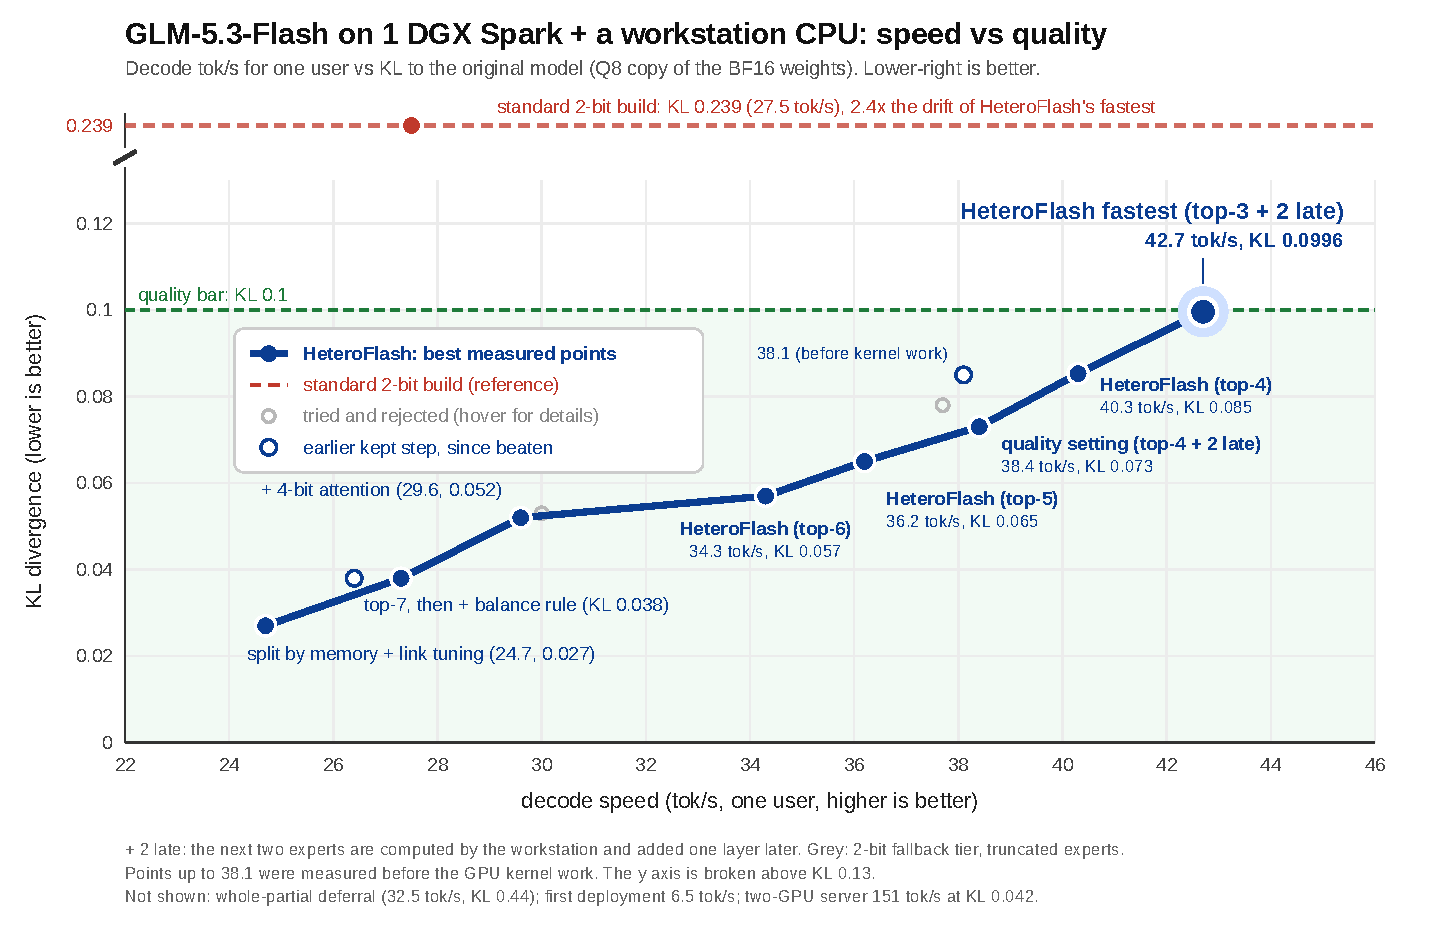
\includegraphics[width=0.86\linewidth]{figures/frontier.pdf}
  \caption{Speed--quality frontier of HeteroFlash on GLM-5.3-Flash (one DGX Spark plus a workstation CPU, one user)
  against the standard 2-bit build that holds every expert on the Spark. Lower right is better.}
  \label{fig:frontier}
\end{figure}

\section{Introduction}
\label{sec:intro}

GLM-5.3-Flash is a mixture-of-experts model: in each of its 42 MoE layers a router picks 8 of 288 routed experts per
token. Only a small part of the model is active per token, but every expert must be readable. At 4 bits the routed
experts alone take about 171--177\,GB, more than one DGX Spark (128\,GB of unified memory) can hold next to the attention
weights, the KV cache and a draft head. The usual answers are more GPUs, or compressing the model so hard (for example
to 2 bits) that its answers get noticeably worse.

We ask: \emph{can GLM-5.3-Flash run interactively (batch 1, one user) on one DGX Spark, helped only by the CPU and RAM of
an ordinary workstation, at quality no worse than a two-GPU server deployment of the same model?}
HeteroFlash answers with a system that pulls four levers on the cost of one decoded token at once
(Figure~\ref{fig:levers}): where each expert runs, how many bits each weight needs, which expert work is worth doing,
and when each piece of work has to finish. A change is kept only if it moves the speed--quality frontier.

\paragraph{Results.} Table~\ref{tab:headline} lists the operating points. The fastest setting computes the 3 strongest
expert picks on time, lets the workstation compute picks 4 and 5 and add them one layer later, and replaces picks 6--8
with each expert's mean output. It decodes 42.7\tps{} at KL 0.0996, against 27.5\tps{} at KL 0.239 for the 2-bit build.
Its top choice disagrees with the full model on 10.0\% of tokens, against 15.1\% for the 2-bit build. Tool calling scored
90/100, against 89/100 for the model with all experts.

\begin{table}[h]
\centering\small
\caption{Operating points on GLM-5.3-Flash, one user, batch 1. KL is to a Q8 copy of the official BF16 weights (lower is
better). top-$k$: experts kept per token out of 8; ``+\,2 late'': the next two experts are computed by the workstation and
added one layer later. Top-6 and top-5 were measured before the GPU kernel work (Section~\ref{sec:res-kernels}), so they
would be somewhat faster today.}
\label{tab:headline}
\begin{adjustbox}{max width=\linewidth}
\begin{tabular}{lccc}
\toprule
setting & decode tok/s & KL & top-1 agreement \\
\midrule
\textbf{HeteroFlash, top-3 + 2 late (fastest)} & \textbf{42.7} & \textbf{0.0996} & 90.0\% \\
HeteroFlash, top-4 + 2 late (quality setting) & 38.4 & 0.073 & 91.5\% \\
HeteroFlash, top-4 & 40.3 & 0.085 & 90.8\% \\
HeteroFlash, top-5 & 36.2 & 0.065 & 92.1\% \\
HeteroFlash, top-6 & 34.3 & 0.057 & 92.8\% \\
Standard 2-bit build, all on the Spark & 27.5 & 0.239 & 84.9\% \\
\midrule
\multicolumn{4}{l}{\emph{References}} \\
Two-GPU workstation server, 3.5-bit EXL3, tensor parallel 2 & 151 & 0.042 & 94.0\% \\
This runtime, all experts on the workstation CPU, no techniques & 15--18 & -- & -- \\
\bottomrule
\end{tabular}
\end{adjustbox}
\end{table}

\paragraph{Contributions.}
\begin{itemize}
  \item A two-machine runtime that computes each routed expert where its weights live: hot experts on the Spark GPU,
    every other expert on the workstation CPU next to its RAM, exchanging only activations and partial sums through an
    in-graph mailbox (Section~\ref{sec:system}). Both memories are read concurrently without interference
    (Section~\ref{sec:res-mem}) and the split is exact (Section~\ref{sec:res-exact}).
  \item A per-step balance rule, mixed precision (Q4\_K experts; NVFP4 attention, shared experts and dense layers; MXFP8
    output head) and latency-oriented link tuning (Section~\ref{sec:methods}).
  \item Rank-aware expert budgets for a single user: top-$k$ truncation without renormalisation, union-aware reuse of
    weak picks inside the speculative verify window, a mean-output stand-in for skipped picks, and weak picks computed
    one layer late on otherwise idle workstation time (Section~\ref{sec:methods}). Union-aware routing is measured on six
    MoE models from three families (Section~\ref{sec:res-union}).
  \item A measured path from 6.5 to 42.7\tps{} (Figure~\ref{fig:steps}) and twelve labelled findings, including
    negative results (Section~\ref{sec:findings}).
\end{itemize}

\section{Background}
\label{sec:background}

\subsection{Mixture-of-experts layers}
In an MoE layer $\ell$ with $N_E$ routed experts, a router produces gate weights for the token's hidden state $x$ and
selects the $k$ highest-scoring experts $\mathcal{T}_\ell(x)$, $|\mathcal{T}_\ell(x)| = k$. The layer output is
\begin{equation}
  y_\ell(x) \;=\; S_\ell(x) \;+\; \sum_{i \in \mathcal{T}_\ell(x)} g_{\ell,i}(x)\, E_{\ell,i}(x),
  \label{eq:moe}
\end{equation}
where $S_\ell$ is the shared expert and $g_{\ell,i}$ is the gate weight of routed expert $i$, normalised over the $k$
original picks. For GLM-5.3-Flash, $N_E = 288$, $k = 8$, and layers 3--44 are MoE layers. Each routed expert is a
gated MLP with hidden size $h = 4096$ and intermediate size $I = 2048$, with the model's clamped SiLU:
\begin{equation}
  E_{\ell,i}(x) \;=\; W^{\mathrm{down}}_{\ell,i}\Big(\operatorname{SiLU}\big(\min(W^{\mathrm{gate}}_{\ell,i}x,\,10)\big)
  \odot \operatorname{clip}\big(W^{\mathrm{up}}_{\ell,i}x,\,-10,\,10\big)\Big).
  \label{eq:expert}
\end{equation}
The per-token cost of~\eqref{eq:moe} is dominated by reading the $k$ selected experts' weights, which is why decoding a
large MoE at batch 1 is bound by memory bandwidth and capacity rather than by arithmetic.

\subsection{Speculative decoding}
Speculative decoding~\citep{specdec} drafts several tokens cheaply and verifies them with the full model in
one pass. GLM-5.3-Flash ships a multi-token-prediction (MTP) draft head. A decode step (``cycle'') here is one verify pass
over a window of $T = 4$ positions plus 3 MTP draft passes. If step $s$ commits $c_s \in \{1,\dots,4\}$ tokens and takes
$t_s$ seconds, single-user decode throughput is
\begin{equation}
  \text{tok/s} \;=\; \frac{\bar c}{\bar t}, \qquad \bar c = \frac{1}{|\mathcal{S}|}\sum_{s\in\mathcal{S}} c_s,\quad
  \bar t = \frac{1}{|\mathcal{S}|}\sum_{s\in\mathcal{S}} t_s .
  \label{eq:toks}
\end{equation}
For example, the fastest point commits $\bar c = 2.95$ tokens per 69.2\ms{} step, about 42.7\tps. Every change in this
report moves either $\bar t$ (faster steps) or $\bar c$ (more accepted draft tokens), and we report both.

The verify window matters for the MoE layers: the 4 positions each pick 8 experts, so the experts that must be read in
layer $\ell$ are the window union $\mathcal{U}_\ell = \bigcup_{t=1}^{T} \mathcal{T}_\ell(x_t)$. Measured per layer and
step, $|\mathcal{U}_\ell| \approx 23.3$ in the base configuration (Section~\ref{sec:placement}).

\subsection{Related systems}
Computing experts on the CPU next to their weights is established practice in hybrid CPU/GPU MoE inference (Fiddler,
KTransformers, HybriMoE~\citep{fiddler,ktransformers,hybrimoe}); hot-expert offloading is studied by Mixtral offloading,
MoE-Infinity and HOBBIT~\citep{mixtraloffload,moeinfinity,hobbit}. Batch-aware expert selection (Lynx~\citep{lynx}) shares
experts across concurrent requests in a batch. The rank-based expert budget, the mean-output stand-in and late weak
picks follow a public expert sensitivity study on Kimi K3.1~\citep{k31study} and a related runtime~\citep{derpseek}.
Co-selection and routing patterns are studied in Patterns behind Chaos, ExFlow and MegaFlux~\citep{chaos,exflow,megaflux}.
We use NVFP4 formats from NVIDIA Model Optimizer~\citep{modelopt}, Spark kernels from the Local Inference Lab vLLM
fork~\citep{lil}, and llama.cpp's Q4\_K and importance-matrix quantization~\citep{llamacpp}.

\section{System design}
\label{sec:system}

\subsection{Hardware}
\label{sec:hardware}

\begin{table}[h]
\centering\small
\caption{Hardware by role.}
\label{tab:hardware}
\begin{tabularx}{\linewidth}{>{\raggedright\arraybackslash}p{2.6cm} L L}
\toprule
role & hardware & what it does \\
\midrule
GPU node & one DGX Spark (GB10, 128\,GB unified LPDDR5X, 273\,GB/s rated) & attention, KV cache, a hot subset of experts, the MTP draft head \\
CPU node & a 32-core, 4-chiplet workstation CPU, 8-channel DDR5-5600, about 230\,GB free RAM; its GPUs are \textbf{not} used at inference & every routed expert in RAM, part of the vocabulary projection, optionally some attention projections \\
link & one direct 10GBASE-T cable, MTU 9000, TCP (no usable RDMA device) & per-layer exchanges \\
control (quality and speed reference) & the same model on a two-GPU workstation server: vLLM, EXL3 3.5\,bpw weights~\citep{exllamav3}, tensor parallel 2, MTP with 3 draft tokens & 151\tps{} prose, and the quality bar of Section~\ref{sec:setup} \\
\bottomrule
\end{tabularx}
\end{table}

The project's targets are 80\tps{} (stretch 120--130) at control quality, a cold 45K-token time to first token (TTFT)
of at most 10.8\,s, and a cached 45K\,+\,32-token TTFT of at most 0.2\,s. \textbf{None of these is met today}
(Section~\ref{sec:limits}).

\subsection{Placement}
\label{sec:placement}

Weights come from the official BF16 release of GLM-5.3-Flash (revision \texttt{f9fed3bbc822}). In the base
configuration the non-expert (``fixed path'') weights run in FP8 on the Spark; the later points
(Sections~\ref{sec:res-stack}--\ref{sec:res-late}) replace FP8 with NVFP4 for attention, shared experts and dense
layers. Every routed expert exists as Q4\_K + importance-matrix GGUF bytes in workstation RAM, and the Spark keeps a
resident hot set of the \emph{same} Q4\_K bytes, so a pick computed on either machine uses identical weights.

A decode cycle is one verify pass over 4 positions plus 3 MTP draft passes. Its work is split three ways:
\begin{itemize}
  \item \textbf{Routed experts (layers 3--44): split by expert, re-balanced every step.} The Spark holds 112--120 hot
    experts per layer, chosen from decode-route counts on a calibration slice disjoint from the measured prompts. Per
    layer and step, an in-graph assign kernel takes the verify window's expert union and runs resident experts on the
    GPU with its own Q4\_K kernel; the rest go to the workstation (balance rule, Section~\ref{sec:balance}). Measured per
    layer and step: a union of 23.3 experts, 12.1 computed on the GPU, 11 on the workstation.
  \item \textbf{Vocabulary projection (lm\_head): split by row.} Rows 0--84,991 on the GPU, the rest on the
    workstation; exact bf16 logits come back (no top-$k$ approximation).
  \item \textbf{Linear-attention (KDA) q/k/v projections: split by head.} Optional; it does not pay (finding F7) and is
    off in the headline configuration.
\end{itemize}
With $P^{G}_\ell$ and $P^{C}_\ell$ the sets of experts assigned to the GPU and to the workstation in this step, layer
$\ell$ computes
\begin{equation}
  y_\ell(x_t) = S_\ell(x_t) + \underbrace{\sum_{i\in\mathcal{T}_\ell(x_t),\, i\in P^{G}_\ell} g_{\ell,i}E_{\ell,i}(x_t)}_{\text{Spark GPU}}
  + \underbrace{\sum_{i\in\mathcal{T}_\ell(x_t),\, i\in P^{C}_\ell} g_{\ell,i}E_{\ell,i}(x_t)}_{\text{workstation CPU, one partial sum}},
  \label{eq:split}
\end{equation}
which is~\eqref{eq:moe} regrouped: the split changes only the summation order and the rounding of the returned partial
sum (bf16 by default).

\subsection{The mailbox exchange}
\label{sec:mailbox}
The GPU stays the master, and the whole step stays inside one CUDA graph:
\begin{enumerate}
  \item A pack kernel writes the layer's routes, gate weights and hidden rows into a pinned, host-mapped mailbox and
    sets a release flag with a device-side sequence counter.
  \item A relay thread on the Spark CPU forwards the request over the direct link to the workstation's expert server
    (32 pinned threads, busy-poll sockets).
  \item A spin-wait kernel queued later in the same graph waits for the reply and adds the workstation's partial sums
    (bf16 by default, fp32 optional).
\end{enumerate}
Exchange points are therefore not graph breaks: about 91 in-graph exchange points per verify pass and 3 per draft pass.
The mailbox is exact against the eager path and under CUDA-graph replay. The design follows published hybrid CPU/GPU MoE
systems (device-visible mailboxes, one captured graph); it is not claimed as new here.

\section{Methods: four levers}
\label{sec:methods}

\begin{figure}[t]
  \centering
  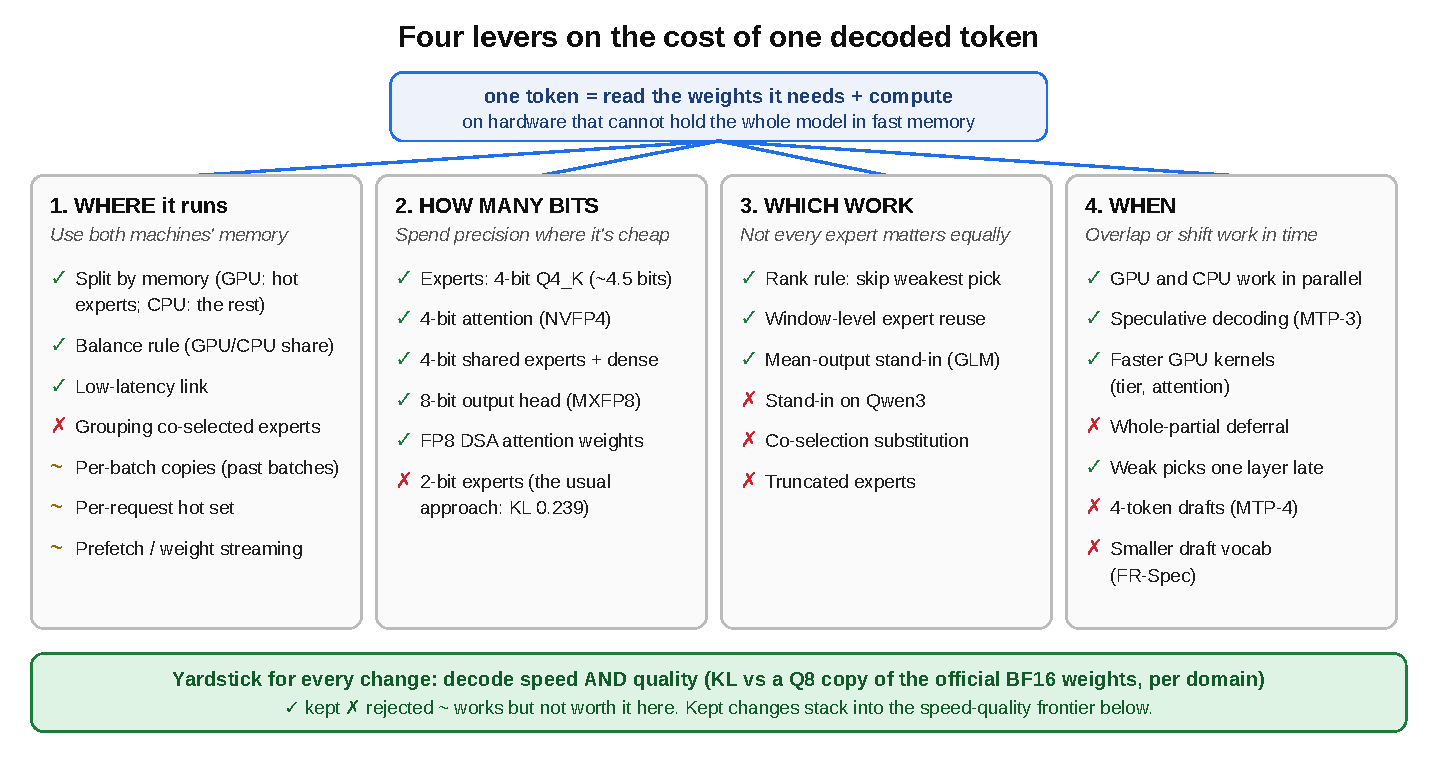
\includegraphics[width=0.86\linewidth]{figures/levers.pdf}
  \caption{The four levers on the cost of one decoded token: where each expert runs, how many bits each weight needs,
  which expert work is worth doing, and when each piece of work has to finish.}
  \label{fig:levers}
\end{figure}

Every decoded token costs the same thing: read the weights it needs, then compute. On hardware that cannot hold the
whole model in fast memory, that leaves four levers (Figure~\ref{fig:levers}).

\subsection{Where each expert runs: the balance rule}
\label{sec:balance}
Let $\mathcal{U}_\ell$ be the set of experts that must be read in layer $\ell$ for the current step: the window union of
the picks that are computed exactly (all picks at top-8; the core union $\mathcal{U}^{\mathcal{C}}$ of
Section~\ref{sec:which} under truncation). Let $U = |\mathcal{U}_\ell|$ and $R = |\mathcal{U}_\ell \cap \mathcal{H}_\ell|$,
the number of those experts that are resident in the GPU hot set $\mathcal{H}_\ell$. The assign kernel walks the
resident experts of $\mathcal{U}_\ell$ in expert-index order and gives the first
\begin{equation}
  \mathrm{cap}_\ell \;=\; \operatorname{clamp}\!\Big(\operatorname{round}(A\,U + B),\; 0,\; \min(R, G_{\max})\Big)
  \label{eq:balance}
\end{equation}
of them to the GPU; all other union experts, resident or not, go to the workstation. $A$ is the balance coefficient
(``A\,0.5'' in the tables), $B$ an offset ($-1$ by default) and $G_{\max}$ the GPU pool limit. The rule is evaluated per
layer and per step inside the CUDA graph, so the split follows the actual routing of each window rather than a static
plan. For several concurrent users a smaller GPU share pays (Section~\ref{sec:res-multi}).

\subsection{How many bits each weight needs}
\label{sec:bits}
Each part of the model gets its own precision, set by how often it is read and how much quality it carries:
routed experts (most of the model's size) in 4-bit Q4\_K, about 4.5 bits per weight with its scales, quantized with an
importance matrix and identical on both machines; attention, shared experts and dense layers (read by every token) in
4-bit NVFP4 (W4A16, round-to-nearest from the BF16 weights), down from FP8; the output head in 8-bit MXFP8. The kv\_b
absorb weights of the 11 DSA attention layers are stored in MXFP8 instead of BF16 (Section~\ref{sec:res-kernels}). Going
lower on the experts, to 2 bits, is the usual way to fit the model on one Spark; it costs 3.7$\times$ more quality than
the top-5 point.

\subsection{Which expert work is worth doing}
\label{sec:which}
For token $t$ in layer $\ell$ let $r_{t,i} \in \{0,\dots,7\}$ be the rank of pick $i$ among the token's 8 picks by gate
weight (ties broken by slot), so rank 0 is the strongest pick.

\paragraph{Top-$K$ truncation and thresholds.} A pick is a \emph{core} pick when
\begin{equation}
  i \in \mathcal{C}_t \iff r_{t,i} < K \;\wedge\; g_{t,i} \ge \tau \sum_{j\in\mathcal{T}(x_t)} g_{t,j},
  \label{eq:core}
\end{equation}
with budget $K \le 8$ and threshold $\tau \ge 0$ (``top-$K$'' points set $\tau = 0$; ``tau'' points set $K = 8$). The
dropped weight is \emph{not} redistributed: the kept picks keep their original top-8 normalisation. The usual alternative
rescales the kept weights by $\sum_{j\in\mathcal{T}} g_{t,j} / \sum_{j\in\mathcal{C}_t} g_{t,j}$; finding F1 shows it is
worse.

\paragraph{Union-aware routing.} In a verify window of $T$ positions the core picks define the experts that must be
read, $\mathcal{U}^{\mathcal{C}} = \{\,e(i) : i \in \mathcal{C}_t,\ t = 1,\dots,T\,\}$, where $e(i)$ is the expert of pick
$i$. A weaker pick is kept if its expert is already in that set:
\begin{equation}
  \mathcal{K}_t \;=\; \mathcal{C}_t \;\cup\; \{\, i \in \mathcal{T}(x_t) \setminus \mathcal{C}_t \;:\; e(i) \in \mathcal{U}^{\mathcal{C}} \,\}.
  \label{eq:union}
\end{equation}
By construction $\bigcup_t \{e(i) : i\in\mathcal{K}_t\} = \mathcal{U}^{\mathcal{C}}$, so the experts read, and hence the
memory traffic, are exactly those of plain top-$K$; the extra tail picks cost only their arithmetic. This applies the
batch-aware selection of Lynx~\citep{lynx}, which shares experts across concurrent requests in a batch, to the speculative
verify window of a single request, where batch-level sharing does nothing.

\paragraph{Mean-output stand-in.} For each layer $\ell$ and expert $e$ we precompute the mean output over calibration
picks $\mathcal{P}_{\ell,e}$ (calibration text, not the evaluation set), using the runtime's own Q4\_K kernel:
\begin{equation}
  \mu_{\ell,e} \;=\; \frac{1}{|\mathcal{P}_{\ell,e}|}\sum_{x\in\mathcal{P}_{\ell,e}} E_{\ell,e}(x) \;\in\; \mathbb{R}^{h}.
  \label{eq:mean}
\end{equation}
A pick that is still skipped contributes its gate weight times this mean instead of nothing. With union-aware routing and
the stand-in, the MoE output is
\begin{equation}
  \hat y_\ell(x_t) \;=\; S_\ell(x_t) \;+\; \sum_{i\in\mathcal{K}_t} g_{t,i}\,E_{\ell,e(i)}(x_t)
  \;+\; \sum_{i\in\mathcal{T}(x_t)\setminus\mathcal{K}_t} g_{t,i}\,\mu_{\ell,e(i)} .
  \label{eq:standin}
\end{equation}
The table holds $42 \times 288$ vectors of size 4096 in 16-bit precision. The stand-in costs one small GPU kernel and no
expert reads.

\subsection{When each piece of work has to finish}
\label{sec:when}
GPU and CPU work overlap within a layer, the link is tuned for latency (finding F6), and speculative decoding commits
about 2.9 tokens per step.

\paragraph{Late weak picks.} With a late depth $D$, the picks ranked just below the on-time budget that are not kept by
union routing,
\begin{equation}
  \mathcal{L}_t \;=\; \{\, i \in \mathcal{T}(x_t)\setminus\mathcal{K}_t \;:\; K \le r_{t,i} < K + D \,\},
  \label{eq:late-set}
\end{equation}
are sent to the workstation in a second request, packed after the layer's main request, and lose the mean stand-in.
Their result
$\Lambda_\ell(x_t) = \sum_{i\in\mathcal{L}_t} g_{t,i}\,E_{\ell,e(i)}(x_t)$ is computed exactly from layer $\ell$'s own MoE
input, but it is added to the output of layer $\ell+1$'s MoE block instead of layer $\ell$'s:
\begin{equation}
  \tilde y_{\ell+1}\big(x_{t}^{(\ell+1)}\big) \;=\; \hat y_{\ell+1}\big(x_{t}^{(\ell+1)}\big) \;+\; \Lambda_\ell\big(x_{t}^{(\ell)}\big),
  \qquad \ell = 3,\dots,43,
  \label{eq:late}
\end{equation}
where $x_t^{(\ell)}$ is the MoE input of layer $\ell$ and $\hat y$ is~\eqref{eq:standin} with $\mathcal{L}_t$ removed
from the stand-in sum. So the late contribution enters the residual stream one layer late: layer $\ell+1$'s attention,
router and experts do not see it, while every later layer does. Picks with rank $\ge K + D$ keep the stand-in, and the
last MoE layer (44) keeps the stand-in for all skipped picks. ``Top-3 + 2 late'' is $K = 3$, $D = 2$: picks 1--3 (and
union picks) on time, picks 4--5 one layer late, picks 6--8 replaced by $\mu$. Because the GPU does not wait for
$\Lambda_\ell$ at layer $\ell$, the late work runs on workstation time that is otherwise idle; it pays only while the
workstation has that slack (finding F12).

\paragraph{Whole-partial deferral.} A coarser variant adds the workstation's entire partial sum of layer $\ell$ (the last
term of~\eqref{eq:split}) one layer late, so the GPU never blocks. It carries strong picks too and fails on quality
(finding F9).

\subsection{The quality constraint}
\label{sec:constraint}
Every change is judged by two numbers, decode speed and quality per domain against a Q8 copy of the official BF16 weights
(Section~\ref{sec:setup}). Writing $\theta$ for a configuration (budget $K$, late depth $D$, precisions, balance rule),
the fastest settings solve
\begin{equation}
  \max_{\theta}\ \text{tok/s}(\theta) \quad\text{s.t.}\quad
  \overline{\KL}(\theta) \le 0.1,\quad \max_{d\in\mathcal{D}} \overline{\KL}_d(\theta) \le 0.15,\quad
  \text{tool}(\theta) \ge 87/100,
  \label{eq:gonogo}
\end{equation}
where $\mathcal{D}$ is the set of 7 evaluation domains (the go/no-go bar). A change is kept only if it moves the
speed--quality frontier; points that trade speed for quality are reported as well.

\section{Experimental setup}
\label{sec:setup}

\paragraph{Speed.} Batch 1, greedy, MTP with 3 draft tokens, CUDA graphs. Each frontier point is a run-time switch on
one server boot, so points run interleaved, round-robin, on the same server. A round sends 15 requests: one 256-token
essay, 4 chat prompts (prose, code, chat, reasoning; 400 tokens) and 10 agent-style items (2 each of tool calling,
multi-turn, coding, prose and reasoning, taken from public benchmarks; 300 tokens; the \texttt{hermes} group in the
result files). For the frontier of Section~\ref{sec:res-frontier} the reported tok/s pools all 15 requests over 3
rounds. The GPU kernel work and late-pick points (Sections~\ref{sec:res-kernels} and~\ref{sec:res-late}) report the
median over interleaved rounds; there, requests hit by a rare multi-second stall (own time per step of 100\ms{} or more)
are left out.

\paragraph{Quality.} A balanced evaluation set of 41 chunks with 41,943 scored tokens in 7 domains (writing/chat,
knowledge QA, math, code, multilingual, instruction following, long context), with prompt \emph{and} answer text. Each
chunk has 2,048 tokens and its second half (1,023 positions) is scored. Every position runs through the split path in
decode-sized batches (16 tokens per step, eager mode). Logits are compared with a Q8\_0 quantization of the BF16 weights
(the ``proxy''). With $p_t$ the run's next-token distribution and $q_t$ the proxy's at scored position $t$, $y_t$ the
actual next token and $N = 41{,}943$,
\begin{align}
  \overline{\KL} &= \frac{1}{N}\sum_{t=1}^{N} \sum_{v\in\mathcal{V}} q_t(v)\,\big(\log q_t(v) - \log p_t(v)\big), \label{eq:kl}\\
  \dNLL &= \frac{1}{N}\sum_{t=1}^{N} \big(-\log p_t(y_t) + \log q_t(y_t)\big), \qquad
  \mathrm{SE}(\dNLL) = \frac{s}{\sqrt{N}}, \label{eq:dnll}\\
  \text{top-1} &= \frac{1}{N}\sum_{t=1}^{N} \mathbb{1}\big[\arg\max\nolimits_v p_t(v) = \arg\max\nolimits_v q_t(v)\big], \label{eq:top1}
\end{align}
where the KL is $\KL(q_t \,\|\, p_t)$ over the full vocabulary $\mathcal{V}$ (proxy probabilities below $e^{-16}$ are
treated as zero), $s$ is the sample standard deviation of the per-token $\dNLL$, and the per-domain
$\overline{\KL}_d$ averages over that domain's positions only. $\dNLL$ is the mean extra negative log-likelihood in nats
per token. Some screens use a 7-chunk subset (one chunk per domain), marked as such. Throughout, ``KL'' in tables means
$\overline{\KL}$.

\paragraph{Two quality bars.} The \emph{control bar} is the two-GPU control's own cost, scored against the same proxy on
the same tokens: $\dNLL = +0.0148$ (SE 0.0017), $\overline{\KL} = 0.042$, top-1 94.0\%. A point is \emph{inside} the
control bar only if all three metrics are at least as good:
\begin{equation}
  \dNLL(\theta) \le 0.0148 \;\wedge\; \overline{\KL}(\theta) \le 0.042 \;\wedge\; \text{top-1}(\theta) \ge 94.0\%.
  \label{eq:controlbar}
\end{equation}
The looser \emph{go/no-go bar}~\eqref{eq:gonogo} (KL at most 0.1, no domain above 0.15, tool calling at least 87/100) is
the one the fastest settings are held to.

\paragraph{Task scores.} Tool calling uses tool-eval-bench~\citep{tooleval} with leaderboard settings. Differences of 2--3
points are within run-to-run noise.

\paragraph{Anchors.} Every speed boot re-runs reference points from the first boot. If an anchor misses by more than
0.3\tps, the boot's other points are not trusted. That rule rejected boot f2 (finding F8). Boot f3 missed it on one
anchor by 0.40\tps, entirely in its cold first round, so its results are reported as same-boot comparisons
(Section~\ref{sec:res-frontier}). Boot d6 (Section~\ref{sec:res-stack}) did not re-run the f1 anchors. Its nearest
cross-boot check, plain top-5 on the same checkpoint, read 35.46\tps{} on d5 and 35.87 on d6 (0.41 apart, just outside
the 0.3 rule), so d6's absolute speeds are $\pm$0.5\tps; its three rounds agree within 0.4\tps.

\section{Results}
\label{sec:results}

\FloatBarrier
\subsection{The two memories add up}
\label{sec:res-mem}
Coordinated, time-stamped streaming on both machines at once (Table~\ref{tab:bw}):

\begin{table}[h]
\centering\small
\caption{Read bandwidth, alone and while the other machine streams.}
\label{tab:bw}
\begin{tabular}{lcc}
\toprule
stream & alone & while the other machine streams \\
\midrule
Spark GPU, bf16 read-reduce & 239.7\,GB/s & 239.8\,GB/s \\
workstation CPU, 32 cores & 251.2\,GB/s & 251.2\,GB/s (Spark GPU \emph{and} Spark Arm cores streaming) \\
\bottomrule
\end{tabular}
\end{table}

The two memories do not interfere, so together they offer about $240 + 251$\,GB/s of raw read bandwidth. Two measured
caveats: the Spark's own Arm cores add nothing, because they share the GPU's memory (a 20-thread Arm stream cut the GPU
from 239.7 to 202\,GB/s); and the workstation CPU is limited by its chiplet links (about 63\,GB/s per chiplet, linear up
to 4), not by DRAM.

A real decode cycle gets less than the sum. In a 90-phase prototype of one verify pass, splitting each layer between the
two machines read \textbf{366\,GB/s effective, against 207\,GB/s for the GPU alone on the same bytes: 56.7 vs 100.1\ms{}
per cycle, 1.77$\times$}. That figure is with Energy-Efficient Ethernet (EEE) and receive coalescing off; at NIC defaults
it was 1.45$\times$.

\FloatBarrier
\subsection{The split is exact}
\label{sec:res-exact}
\begin{itemize}
  \item \textbf{In math.} Splitting real FP8 attention layers by head across the two machines matches the unsplit
    computation to $1.1\times10^{-6}$ (linear-attention layer) and $7.8\times10^{-7}$ (MLA layer) relative $L_2$ in fp32.
  \item \textbf{Kernels.} The Spark's Q4\_K expert kernel matches an fp32 dequantized reference to
    $3\text{--}6\times10^{-7}$ relative $L_2$.
  \item \textbf{End to end, paired on the same 40,920 tokens.} Unsplit vs split with bf16 partial sums:
    $\dNLL = +0.0007$ (SE 0.0008), direct KL 0.010, same top-1 96.9\%. For scale, 96.8--97.0\% top-1 agreement is what
    summation order alone produces between any two of these runs, and fp32 vs bf16 partial sums differ by $-0.0007$
    (SE 0.0008). The split against the proxy: $+0.0044$ (SE 0.0014), KL 0.027, top-1 95.1\%, well inside the control bar.
\end{itemize}

\FloatBarrier
\subsection{Speed progression}
\label{sec:res-progression}

\begin{figure}[t]
  \centering
  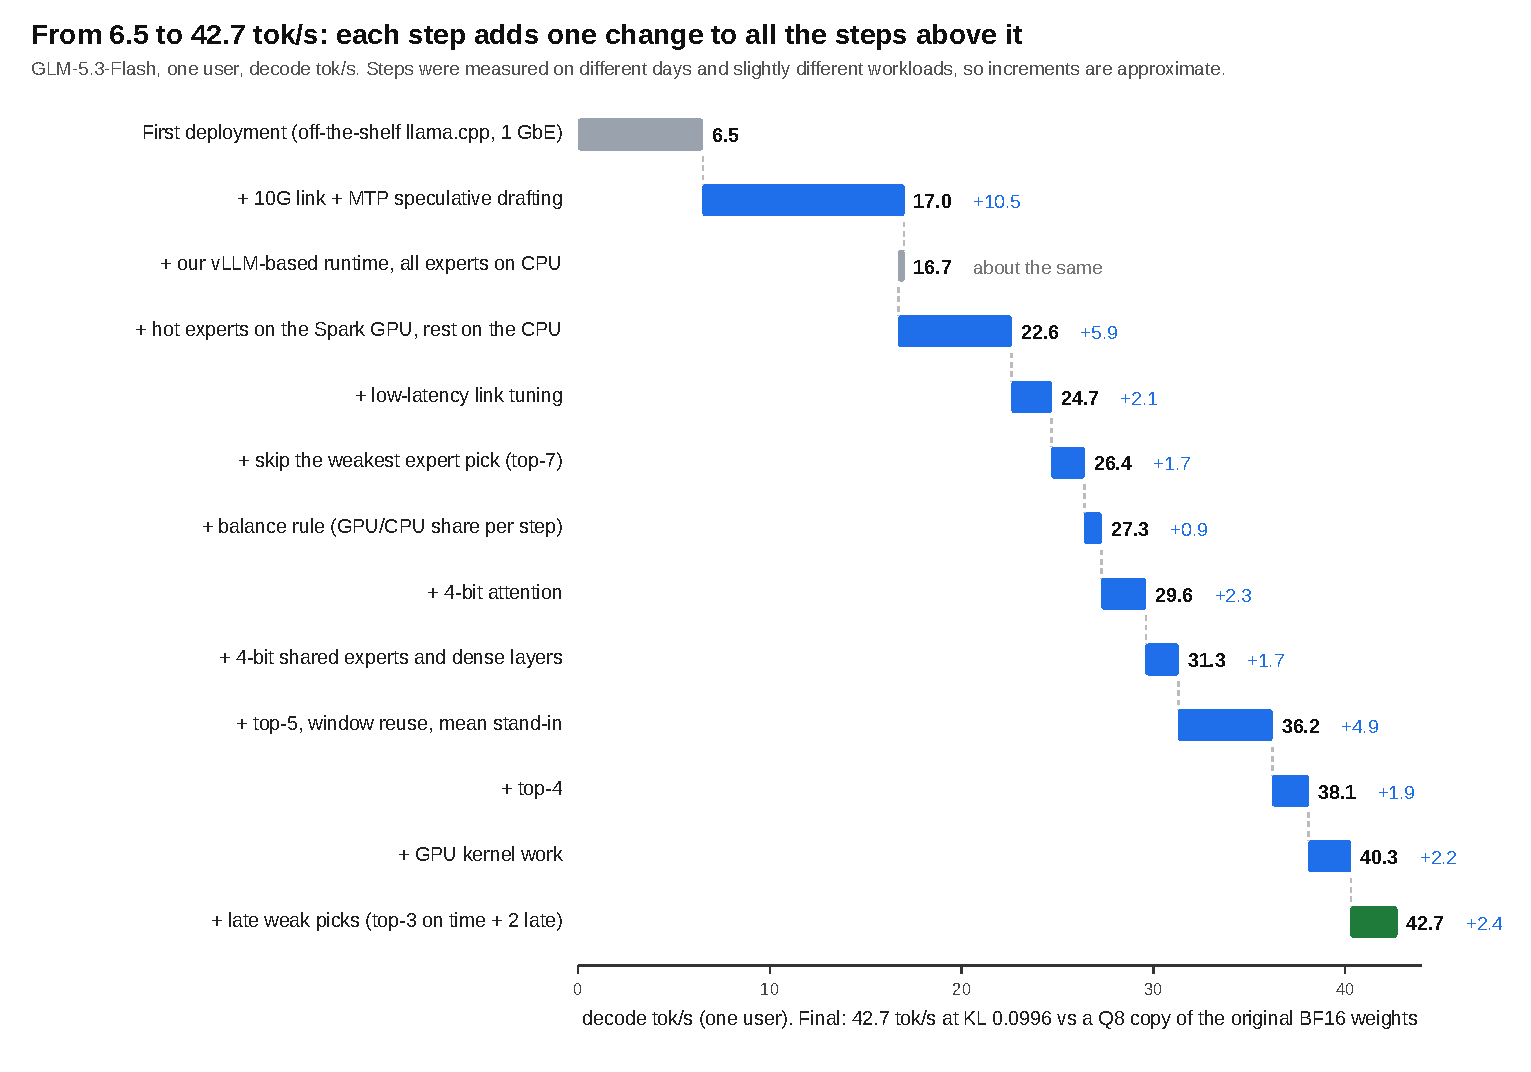
\includegraphics[width=0.92\linewidth]{figures/speed_steps.pdf}
  \caption{Cumulative steps from 6.5 to 42.7\tps. Each row adds one change on top of all the rows above it. Rows were
  measured on different boots and slightly different workloads, so the increments are approximate, not a clean
  ablation.}
  \label{fig:steps}
\end{figure}

Table~\ref{tab:steps} summarises the cumulative path of Figure~\ref{fig:steps}; Table~\ref{tab:progression} gives the
early stages with their workloads. Rows of Table~\ref{tab:progression} use different workloads, so compare within a
group of rows, not across groups.

\begin{table}[h]
\centering\small
\caption{Cumulative steps (each adds one change to all rows above it).}
\label{tab:steps}
\begin{tabularx}{\linewidth}{>{\raggedright\arraybackslash}p{4.1cm} L >{\centering\arraybackslash}p{1.9cm} >{\centering\arraybackslash}p{1.6cm}}
\toprule
step & what this step means & tok/s & KL \\
\midrule
first deployment & off-the-shelf llama.cpp splitting the model's layers between the two machines over 1\,GbE, no speculative decoding & 6.5 & \\
+ 10G link + MTP drafting & a faster cable; the draft head guesses 3 tokens ahead & 17.0 & \\
+ vLLM runtime, all experts on the workstation CPU & our vLLM-based runtime; about the same speed, but the base for the split & 15--18 (16.7 average) & \\
+ split by memory & hot experts on the Spark GPU, the rest on the workstation CPU & 22--23 & 0.027 \\
+ low-latency link tuning & link power saving and interrupt batching off; attention no longer split & 24.7 & 0.027 \\
+ skip the weakest pick (top-7) & 7 of 8 experts per token & 26.4 & 0.038 \\
+ balance rule & per-step GPU/CPU expert split, Eq.~\eqref{eq:balance} & 27.3 & 0.038 \\
+ 4-bit attention & attention weights in NVFP4 instead of FP8 & 29.6 & 0.052 \\
+ 4-bit shared experts and dense layers & the same for the parts every token uses & 31.3 & $\approx$ same \\
+ top-5, window reuse, mean stand-in & Eqs.~\eqref{eq:union}--\eqref{eq:standin} & 36.2 & 0.065 \\
+ top-4 & 4 of 8 experts & 38.1 & 0.085 \\
+ GPU kernel work & parallel tier kernel, FP8 DSA kv\_b + GEMV, KDA projection GEMV & 40.3 & 0.085 \\
+ late weak picks (top-3 + 2 late) & Eq.~\eqref{eq:late} with $K=3$, $D=2$ & \textbf{42.7} (+2.4) & \textbf{0.0996} \\
\bottomrule
\end{tabularx}
\end{table}

\begin{table}[h]
\centering\small
\caption{Early speed progression with workloads. Sources in Appendix~\ref{app:artifacts}.}
\label{tab:progression}
\begin{tabularx}{\linewidth}{L >{\raggedright\arraybackslash}p{2.4cm} >{\raggedright\arraybackslash}p{3.6cm}}
\toprule
stage & workload & tok/s \\
\midrule
control, two-GPU server & prose & 150.8 \\
first end-to-end deployment (llama.cpp RPC over 1\,GbE, no drafting) & prose & 6.46 \\
same, direct 10G link + MTP drafting & prose & 17.0 \\
``config B'': vLLM, FP8 fixed path, \textbf{all} routed experts on the workstation CPU, mailbox, MTP-3 (3 reps) & essay / chat / agent & 16.58 / 15.43 / 18.00 \\
dual-memory split, same session (3 reps) & essay / chat / agent & 22.82 / 22.05 / 23.03 \\
frontier boot f1: split, KDA split on & 15-request pool & 20.75 (21.8 on warm rounds 2--3) \\
f1: KDA split off (lossless) & 15-request pool & 23.21 \\
f1: KDA split off + workstation NIC interrupt coalescing off (lossless) & 15-request pool & 24.68 (6 rounds, ABBA) \\
\textbf{f3: top-7 experts + KDA split off (earlier operating point)} & 15-request pool & \textbf{25.62} (25.7 on warm rounds 2--3, derived) \\
\bottomrule
\end{tabularx}
\end{table}

The split against config B in the same session: cycle time 148.5 to 120.6\ms{} (essay) and 150.9 to 119.9\ms{} (chat),
1.21--1.26$\times$. For context, the Spark alone, with every expert in 2 bits on the GPU, reaches about 27--28\tps{} but
scores $\dNLL = +0.18$ against the proxy, twelve times the control's $+0.0148$. The workstation is what buys the quality.

\FloatBarrier
\subsection{The speed--quality frontier of expert dropping}
\label{sec:res-frontier}
The lever: drop routed experts at run time, either with a fixed top-$k$ (keep the $k$ highest-scoring of the 8) or with
a weight threshold $\tau$ (drop experts whose gate weight is below $\tau$ times the sum), Eq.~\eqref{eq:core}. The
dropped weight is not redistributed. All points have the KDA split off. Speed is pooled tok/s over 3 interleaved rounds.

\begin{table}[h]
\centering\small
\caption{Frontier of plain expert dropping (FP8 fixed path, no union, no stand-in).}
\label{tab:frontier}
\setlength{\tabcolsep}{4pt}
\begin{tabularx}{\linewidth}{>{\raggedright\arraybackslash}p{3.0cm} >{\raggedright\arraybackslash}p{2.9cm} cccL}
\toprule
point & tok/s (boot) & $\dNLL$ (SE) & KL & top-1 & against the control bar \\
\midrule
control bar & & +0.0148 (0.0017) & 0.042 & 94.0\% & \\
all 8 experts (lossless reference) & 23.2 (f1); 23.9 (f3, rounds 2--3, derived) & +0.0044 (0.0014) & 0.027 & 95.0\% & inside \\
$\tau = 0.04$ & 24.3 (f3) & +0.0055 (0.0014) & 0.030 & 94.9\% & inside \\
\textbf{top-7} & \textbf{25.6 (f3)} & \textbf{+0.0099 (0.0016)} & \textbf{0.037} & \textbf{93.9\%} & dNLL and KL inside; top-1 0.1\,pt under \\
top-7 + $\tau = 0.04$ & 25.8 (f3) & +0.0112 (0.0017) & 0.040 & 93.8\% & top-1 0.2\,pt under \\
top-6 & 25.8 (f1) & +0.0181 (0.0020) & 0.059 & 92.4\% & outside \\
$\tau = 0.08$ & 26.4 (f1); 26.3 (f3) & +0.0313 (0.0022) & 0.077 & 91.4\% & outside \\
top-4 & 27.6 (f1) & +0.0886 (0.0031) & 0.156 & 86.9\% & far outside \\
top-4, weights renormalised & not timed & +0.1234 (0.0034) & 0.174 & 86.6\% & far outside \\
\bottomrule
\end{tabularx}
\end{table}

Timed but not quality-scored (past the bar by construction, since each drops more than a scored point that is already
outside): top-5 27.1, top-6 + $\tau$ 0.08 27.6, top-4 with 3-bit experts on 15 CPU layers 28.0, top-4 + coalescing off
30.4\tps{} (all f1).

\paragraph{Earlier operating point: top-7 with the KDA split off, 25.7\tps{} on warm rounds} (25.62 pooled, including
the cold first round; superseded by Sections~\ref{sec:res-nvfp4} and~\ref{sec:res-stack}). Boot f3 missed the 0.3\tps{}
anchor rule on one anchor, so these are same-boot comparisons. That is about +7.5\% over lossless on the same boot (23.9,
derived from rounds 2--3) and +10\% over f1's lossless 23.2. $\dNLL$ and KL are inside the control bar. Same-top-1 is
93.88\% against the control's 93.97\%, so it fails the strict all-three rule~\eqref{eq:controlbar} by 0.1 point; with a
top-1 standard error of about 0.12 point we read it as \emph{at} the bar, not inside it. Top-7 combined with coalescing
off is \emph{modeled} at about 27\tps; it has not been measured.

\FloatBarrier
\subsection{NVFP4 attention, deferral and union-aware routing}
\label{sec:res-nvfp4}
All points: speculative mode MTP-3, batch 1, KV cache pinned, a warm-up point plus 3 interleaved rounds per boot.
Quality uses the same balanced evaluation, full (41 chunks) or the 7-chunk subset, as marked.

\begin{table}[h]
\centering\small
\caption{Speed (tok/s, same-boot comparisons). ``A 0.5'': balance rule~\eqref{eq:balance} with $A = 0.5$.}
\label{tab:d3d4}
\begin{tabular}{llcccc}
\toprule
boot & fixed path & top-7 & top-7, A 0.5 & top-6, A 0.5 & top-5, A 0.5 \\
\midrule
d3 & FP8 & 26.37 & 27.33 & 27.85 & 30.08 \\
d4 & NVFP4 attention (W4A16) & & 29.56 & 32.17 & 33.36 \\
\bottomrule
\end{tabular}
\end{table}

\begin{table}[h]
\centering\small
\caption{Quality, full evaluation (41 chunks). ``Weak picks one layer late'' here is the first late-pick test, before
the GPU kernel work; Section~\ref{sec:res-late} has the current late path.}
\label{tab:dq}
\begin{adjustbox}{max width=\linewidth}
\begin{tabular}{lcccl}
\toprule
point & $\dNLL$ (SE) & KL & top-1 & worst domain \\
\midrule
FP8, top-7 & +0.0096 (0.0016) & 0.038 & 94.0\% & instruction following 0.060 \\
NVFP4 attention, top-7 & +0.0183 (0.0019) & 0.052 & 93.0\% & instruction following 0.084 \\
NVFP4 attention, top-5 + weak picks one layer late & +0.0247 (0.0021) & 0.062 & 92.3\% & knowledge QA 0.081 \\
NVFP4 attention, top-4 + weak picks one layer late & +0.0362 (0.0024) & 0.079 & 91.2\% & knowledge QA 0.107 \\
\bottomrule
\end{tabular}
\end{adjustbox}
\end{table}

\FloatBarrier
\subsection{The full stack behind the top-6/5/4 points}
\label{sec:res-stack}
Checkpoint \texttt{mixed\_full\_iq2xxs\_nvfp4attn\_sd}: W4A16 NVFP4 for attention, shared experts and the dense MLP
layers (round-to-nearest from the official BF16 weights with our converter), lm\_head MXFP8, routed experts Q4\_K on
both machines. Runtime: union-aware routing~\eqref{eq:union} plus the mean-output stand-in~\eqref{eq:standin}, with the
mean table built from calibration text, not the evaluation set. Balance rule A 0.5. Speed: boot d6, MTP-3, KV cache
pinned, warm-up plus 3 interleaved rounds.

\begin{table}[h]
\centering\small
\caption{Full stack: speed (boot d6) and quality (full evaluation, 41 chunks).}
\label{tab:stack}
\setlength{\tabcolsep}{4pt}
\begin{adjustbox}{max width=\linewidth}
\begin{tabular}{lccc|cccl}
\toprule
point & tok/s & ms/cycle & tokens/cycle & $\dNLL$ (SE) & KL & top-1 & worst domain \\
\midrule
top-6 + union + stand-in & 34.34 & 85.5 & 2.94 & +0.0181 (0.0020) & \textbf{0.057} & 92.8\% & instr.\ following 0.086 \\
top-5 + union + stand-in & 36.16 & 80.0 & 2.89 & +0.0188 (0.0021) & \textbf{0.065} & 92.1\% & instr.\ following 0.101 \\
top-4 + union + stand-in & 38.12 & 75.5 & 2.88 & +0.0320 (0.0024) & 0.085 & 90.7\% & instr.\ following 0.134 \\
\bottomrule
\end{tabular}
\end{adjustbox}
\end{table}

At top-6 every domain is within 0.1. The same checkpoint without union or stand-in (boot d5): top-7 31.32, top-6 32.73, top-5 35.46\tps.

\paragraph{What the stand-in and union each buy} (7-chunk subset, NVFP4-attention checkpoint, same boot): top-5 plain
KL 0.085, + stand-in 0.056, + union + stand-in 0.045; top-4 + stand-in 0.081, + union + stand-in 0.063. On this model
the stand-in roughly halves the cost of the dropped picks. It does not transfer to Qwen3-30B-A3B, where it is neutral to
slightly worse (Table~\ref{tab:rejected}).

\paragraph{The 2-bit comparison point} (all routed experts IQ2\_XXS on the Spark GPU, same evaluation and scorer): KL
0.239, top-1 84.9\%, $\dNLL = +0.183$, at about 27--28\tps. $0.239 / 0.065 = 3.7$.

\paragraph{Tool calling} (tool-eval-bench, leaderboard settings): 90/100 for top-5 + union + stand-in vs 89/100 for the
all-8-experts FP8 baseline. The difference is within run-to-run noise, so we read it as matching the baseline. Decode on
the same benchmark: 28.1 vs 20.8\tps.

\FloatBarrier
\subsection{GPU kernel work}
\label{sec:res-kernels}
Same checkpoint and routing as top-4 in Section~\ref{sec:res-stack}, plus three GPU changes on the Spark: a parallel tier
kernel (the per-layer decision of which expert runs where), MXFP8 weights with a small-batch GEMV for the DSA attention
kv\_b absorb, and a small-batch GEMV for the KDA attention projections on their existing NVFP4 bytes. Speed is the median
over interleaved rounds, with stalled requests left out (Section~\ref{sec:setup}).

\begin{table}[h]
\centering\small
\caption{GPU kernel work at top-4 + union + stand-in.}
\label{tab:kernels}
\begin{adjustbox}{max width=\linewidth}
\begin{tabular}{lcccc}
\toprule
point & tok/s & ms per step & committed tokens per step & rounds \\
\midrule
reference, same day (serial tier kernel) & 36.4 & 77.3 & 2.82 & 3 \\
+ parallel tier kernel & 37.6 & 75.4 & 2.84 & 3 \\
+ DSA kv\_b MXFP8 + KDA projection kernel (final) & \textbf{40.3} & \textbf{72.0} & 2.90 & 5 \\
\bottomrule
\end{tabular}
\end{adjustbox}
\end{table}

\begin{itemize}
  \item At equal acceptance, 77.3 to 72.0\ms{} per step is about +7\%. The rest of the +11\% comes from more committed
    tokens per step (2.82 to 2.90), which is within the drift seen between identical boots. In terms of~\eqref{eq:toks},
    the first part is a $\bar t$ gain and the second a $\bar c$ gain.
  \item The parallel tier kernel replaced one GPU thread looping over all 288 experts with one thread per expert:
    38\,\textmu s to 3.7\,\textmu s per layer, about 1.9\ms{} per step, output identical (checked on 59,808 live decode
    windows). It sits ahead of every workstation exchange, so its time is on the critical path.
  \item The kv\_b weights of the 11 DSA attention layers in MXFP8 instead of BF16, with a kernel written for 1--4 tokens:
    about 2.1\ms{} per step faster, KL +0.0006. The KDA projection GEMV: about 1.2\ms{} per step, lossless (same weight
    bytes).
  \item Full evaluation (41 chunks), same boot: KL 0.0856 to 0.0853; worst domain instruction following 0.134 to 0.132.
    Tool calling at top-4 scored 89/100, the same as the all-experts baseline; that run was before the kernel work,
    which leaves KL unchanged.
  \item Not kept: an NVFP4 MTP eh\_proj (about 1\ms{} per step saved, but acceptance fell, so tok/s was flat), NVFP4 kv\_b
    (same speed as MXFP8 at 5$\times$ the KL increase), and the smaller FR-Spec draft head (Section~\ref{sec:negative}).
\end{itemize}

Where each 72--76\ms{} top-4 step went: about 85\% is Spark GPU work (attention, the GPU-resident experts, the draft
head). The GPU waits on the workstation only about 11\ms{} per step, the workstation CPU is about 40\% busy, and the
network is 19\% of each round trip. The late path of the next section uses that spare workstation time: one pick fewer
on time, two late picks on the workstation, 69\ms{} per step.

\FloatBarrier
\subsection{Late weak picks: the current best}
\label{sec:res-late}
Same as Section~\ref{sec:res-kernels}, plus the late path of Eq.~\eqref{eq:late}: after the per-layer tier decision,
picks ranked just below the on-time budget are sent to the workstation in a second request, packed after the main one,
and their result is added after the next layer's experts. Picks past the late budget keep the mean stand-in; union picks
stay on time. Speed: median of interleaved rounds against top-4 on the same boot; quality: full evaluation (41 chunks).

\begin{table}[h]
\centering\small
\caption{Late weak picks. The tok/s column gives the point and, in parentheses, top-4 on the same boot.}
\label{tab:late}
\setlength{\tabcolsep}{3.5pt}
\begin{adjustbox}{max width=\linewidth}
\begin{tabular}{lllccccc}
\toprule
point & on time & one layer late & tok/s (top-4) & ms/step & KL & worst domain & top-1 \\
\midrule
top-4 (reference) & top-4 + union & -- & 39.7 & 72.1 & 0.0853 & instr.\ following 0.132 & 90.8\% \\
\textbf{top-3 + 2 late} & top-3 + union & picks 4--5 & \textbf{42.7} (39.7), +7.6\% & 69.2 & \textbf{0.0996} & instr.\ following 0.137 & 90.0\% \\
top-4 + 2 late & top-4 + union & picks 5--6 & 38.4 (40.0), $-$4.0\% & 74.0 & 0.073 & knowledge QA 0.102 & 91.5\% \\
top-3 + 3 late & top-3 + union & picks 4--6 & 38.3 (40.0), $-$4.2\% & 75.6 & not run & & \\
top-4 + 4 late & top-4 + union & picks 5--8 & 32.5 (40.0), $-$18.6\% & 88.2 & not run & & \\
\bottomrule
\end{tabular}
\end{adjustbox}
\end{table}

\begin{itemize}
  \item \textbf{How the 42.7\tps{} was measured.} Median of 3 interleaved rounds on a fresh server boot: 69.2\ms{} per
    decode step and 2.95 tokens committed per step, against 39.7\tps{} (72.1\ms) for top-4 on the same boot: +7.6\%.
    An earlier boot gave 42.4 vs 39.2\tps{} (+8.2\%), so the gain repeats. About half of it is faster steps (72.1 to
    69.2\ms, about +4\%); the rest is more committed tokens per step (2.86 to 2.95), seen on both boots. The point is
    top-3 + union routing on time, picks 4 and 5 computed by the workstation and added one layer later, the mean
    stand-in for picks 6--8, and the GPU kernel work.
  \item \textbf{Why it pays now.} The earlier test (Table~\ref{tab:dq}, finding F12) ran while the workstation's page
    cache was thrashing. With a healthy expert server the workstation is about 40\% busy and the GPU waits about 11\ms{}
    per top-4 step, so two late picks fit in that slack. Four late picks overload it: the GPU waits 27\ms{} per window
    instead of 10.
  \item \textbf{Quality.} KL 0.0996 and worst domain 0.137 pass the go/no-go bar~\eqref{eq:gonogo} (KL at most 0.1, no
    domain above 0.15) by a thin margin. Top-4 + 2 late is better than plain top-4 in every domain (worst knowledge QA
    0.102).
  \item \textbf{Tool calling} (same boot): top-3 + 2 late 90/100, top-4 88/100; the all-experts baseline scored 89/100.
    Top-4 + 2 late has no run of its own.
  \item \textbf{Not kept.} Top-3 + 1 late was faster still (+9.8\%), but its subset quality, scaled to the full
    evaluation, missed the bar. Putting GPU-resident weak picks on the GPU and only the rest late was slower ($-$7.7\% at
    top-3, $-$19.4\% at top-4).
\end{itemize}

\FloatBarrier
\subsection{Union-aware routing on other models}
\label{sec:res-union}
To test whether union-aware routing~\eqref{eq:union} generalises, we use fewer experts per token two ways on five more
MoE models, plain (drop everything below the top-$K$) and union-aware, at the same number of expert reads. Quality cost
is full-vocabulary KL to the unmodified model (all experts) on the same text: teacher-forced 128-token chunks of a
7-domain evaluation set (168 chunks per model), vLLM on two RTX PRO 6000 GPUs. The share of the quality loss from
dropping experts that union routing removes is
\begin{equation}
  \delta \;=\; 1 - \frac{\overline{\KL}_{\text{union}}}{\overline{\KL}_{\text{plain}}} .
  \label{eq:lessdamage}
\end{equation}

\begin{table}[h]
\centering\small
\caption{Union-aware vs plain truncation at equal expert reads.}
\label{tab:union}
\setlength{\tabcolsep}{4pt}
\begin{adjustbox}{max width=\linewidth}
\begin{tabular}{llccc}
\toprule
model & experts, top-$k$ & union / plain KL (top-6 / 5 / 4) & $\delta$ & union better on \\
\midrule
Qwen3-30B-A3B & 128, top-8 & 0.64 / 0.63 / 0.61 & 36\% / 37\% / 39\% & 162--165 of 168 chunks \\
Qwen3.6-35B-A3B & 256, top-8 & 0.72 / 0.69 / 0.68 & 28\% / 31\% / 32\% & 155--166 of 168 \\
gpt-oss-120b & 128, top-4 & 0.68 (top-3) / 0.74 (top-2) & 32\% / 26\% & 151 / 147 of 168 \\
GLM-4.5-Air (106B) & 128, top-8 & 0.78 / 0.71 / 0.70 & 22\% / 29\% / 30\% & 149--162 of 168 \\
Qwen3.8-Flash-Next (180B) & 512, top-10 & 0.87 / 0.80 / 0.78 (top-8 / 6 / 5) & 13\% / 20\% / 22\% & 136--160 of 168 \\
\bottomrule
\end{tabular}
\end{adjustbox}
\end{table}

Union adds at most 0.05 expert reads per 4-token window, so speed is unchanged. Union helps on every model, but the size
varies; the gain tracks how many dropped picks the window recovers (42\% of them on Qwen3-30B, 23--34\% on the others),
and models with more experts share fewer experts between neighbouring tokens. Size, expert count, family and
quantization change together across these models, so no single cause is isolated. gpt-oss-120b is measured at 128
tokens only: its long-context path gave unusable reference outputs in this vLLM build on these GPUs. In the HeteroFlash
runtime itself (GLM-5.3-Flash, 288 experts; different setup and chunks, so not directly comparable), union routing
removed 24\% / 24\% / 31\% of the loss at top-6 / 5 / 4. Every reference run through the hook reproduces the unmodified
model exactly (KL 0); deterministic MoE kernels are used where the default kernels varied between identical runs. On
Qwen3.6-35B, GSM8K at top-2 rose from 91.1\% to 93.9\% with union routing; plain top-3 matches union at top-2, so the gain
is fewer expert reads, not accuracy per expert computed.

\FloatBarrier
\subsection{Several users at once}
\label{sec:res-multi}
Concurrency $C = 1, 2, 4$ users at top-4, measured before the GPU kernel work (8 prompts of 512 tokens per run, about
100 runs per setting):

\begin{table}[h]
\centering\small
\caption{Multi-stream decode at top-4.}
\label{tab:multi}
\begin{tabular}{cccc}
\toprule
concurrency $C$ & total tok/s & per user & GPU share of each step's experts \\
\midrule
1 & 36.7 & 36.7 & 50\% \\
2 & 47.6 & $\sim$24 & 35\% \\
4 & 50.5 & $\sim$12.6 & 15\% \\
\bottomrule
\end{tabular}
\end{table}

With the single-user split (GPU takes half), 4 users were slower in total than one (28.2\tps). The Spark's expert kernel
re-reads each expert's weights for every group of 4 tokens, so its cost grows with the number of users, while the
workstation handles big batches well; moving more of the work to the workstation fixes most of it (2 users: 39.6 to
47.6). Distinct experts per layer grow from about 12 (1 user) to 41 (4 users). Quality does not depend on the split: it
only moves the same Q4\_K experts between the two machines, and tool calling with 4 conversations in parallel scored
89/100. A step with more than 16 tokens falls back to a slower all-workstation path, so $C = 8$ or 10 is not measured.

\section{Findings and negative results}
\label{sec:findings}
Each finding is labelled. \emph{Likely new} means we did not find it stated in the prior work we checked; it is not a
claim that nobody has seen it. \emph{Known} means established practice or published; those are listed because the
measured size matters here.

\finding{F1. Renormalising after dropping experts hurts.}{Likely new as a measured ablation.}
The usual implementation divides the kept experts' gate weights by their sum, so they add up to 1 again. Leaving the
dropped mass out instead (Eq.~\eqref{eq:core}) was better at every level we measured:
\begin{itemize}
  \item Model level, frontier evaluation: top-4 renormalised $+0.1234$ vs plain top-4 $+0.0886$ $\dNLL$.
  \item Layer level, real inputs: renormalised top-4 output error 0.23--0.69 per layer, against 0.05--0.47 with the
    original top-8 normalisation. The latter is within 0.011 of the least-squares-optimal weights for the same 4 experts.
  \item An earlier model-level run on a different evaluation set agrees: 0.257 vs 0.205 nats.
\end{itemize}
Related work on dynamic expert skipping exists; we found no direct renormalised-vs-not ablation in it.

\finding{F2. Fixed top-$k$ beat a weight threshold at matched speed.}{Setting-specific; likely new for this model.}
On the same boot, top-6 gave 25.8\tps{} at $+0.0181$ $\dNLL$, while $\tau = 0.08$ gave 26.4\tps{} at $+0.0313$: about
1.7$\times$ the quality cost for +0.6\tps. The gentle threshold $\tau = 0.04$ was nearly free ($+0.0055$ vs $+0.0044$)
but bought only +0.4\tps{} (+1.6\%), inside the $\pm$0.5\tps{} measurement band. It saves little because it drops
little: 0.33 of 8 experts per token (1\% of the gate weight), and it shrank the 4-position expert union by 4.3\%
(GPU-only screen). Why $\tau = 0.08$ costs more quality than top-6 at similar speed is not established. Caveat: only two
thresholds were tested; published threshold policies on other models report good frontiers.

\finding{F3. A cycle floor of about 100--115\ms{} capped what dropping experts could buy; overlap was the next lever.}{The
floor is measured; the conclusion is our inference.}
Within the control bar, trading accuracy bought +7--10\% (23.2--23.9 to 25.7\tps). Even top-4, far past the bar, only
reached a 100\ms{} cycle (100.2\ms{} at 2.77 committed tokens per cycle). The floor is made of sequential exchanges. Each
expert exchange costs 0.91\ms{} of server compute but 1.23\ms{} round trip, so about 0.32--0.36\ms{} per exchange is
outside compute. With $n_x \approx 80$ exchanges per cycle that is
\begin{equation}
  n_x\,\big(t_{\text{rtt}} - t_{\text{server}}\big) \;\approx\; 80 \times 0.32\text{--}0.36\ms \;\approx\; 26\ms
  \text{ per cycle (derived)},
  \label{eq:floor}
\end{equation}
on top of the CPU expert time itself. Dropping experts shortens neither the per-exchange latency nor the number of
exchanges, so the next speedups had to come from overlapping the exchange with GPU work, or from fewer, fused exchanges.

\finding{F4. The two memories really are additive, and the Spark's Arm cores are not a third tier.}{The concept is known
(hybrid CPU/GPU MoE inference); the measurements are new for this pair.}
Section~\ref{sec:res-mem}: 239.8 + 251.2\,GB/s concurrently, 1.77$\times$ effective in a full-cycle prototype; a
20-thread Arm stream takes 16\% of the Spark GPU's bandwidth.

\finding{F5. Splitting by head, expert or vocabulary row is exact, and bf16 partial sums cost nothing measurable.}{Known
technique (tensor-parallel-style decomposition); validated here.}
See Section~\ref{sec:res-exact}. A pre-registered per-layer criterion (split vs GPU-only error at most $10^{-3}$) was
\textbf{not} met ($2.3\text{--}3.0\times10^{-3}$). A control that splits the same heads across two GPU runs, with no CPU
involved, gives the same $2.3\text{--}2.5\times10^{-3}$, so the gap is bf16 output rounding: the criterion was set below
bf16 resolution.

\finding{F6. Turning NIC interrupt coalescing off is a lossless lever, and so is turning Energy-Efficient Ethernet off.}{Known
low-latency networking practice; the size of the effect is the result.}
Workstation receive interrupt coalescing off (ABBA order, same boot): cycle 122.8 to 115.5\ms, 23.3 to 24.7\tps{} at
full quality; 99.9 to 91.3\ms, 27.8 to 30.4\tps{} at top-4. It changes no arithmetic, so quality is unchanged. An early
$\sim$300\,\textmu s ``idle-gap penalty'' per exchange turned out to be EEE: any quiet gap longer than the NIC's
low-power-idle timer (115\,\textmu s) puts the link to sleep, and waking it costs about 150--250\,\textmu s. With EEE
off, 90 swaps per cycle took 5.6\ms{} instead of 15--18\ms. Where EEE must stay on, a software keep-alive byte during
idle gaps recovers part of it.

\finding{F7. Splitting the linear-attention projections does not pay.}{Measured; specific to this runtime.}
On the same boot, turning the KDA head split off raised throughput from 21.8 to 23.2\tps{} on warm rounds (+6\%; pooled
20.75 to 23.21, where the pooled split-on figure includes that boot's cold first round), with no quality change. The split
adds one exchange per linear-attention layer (34 per pass), and that latency costs more than the bandwidth it saves. The
vocabulary-projection split, one large exchange, is kept; its own benefit was not resolved beyond trajectory noise in a
1-rep comparison.

\finding{F8. Two benchmark pitfalls: KV-cache size variance and cold first rounds.}{Known classes of problem, stated because
they nearly produced wrong conclusions here.}
\emph{KV-cache size.} One boot came up with a 230,589-token KV cache instead of 302,193 at the same memory-utilisation
setting (non-torch memory +1.8\,GiB; the cause is unexplained). Long agent prompts were then evicted from the prefix
cache (hit rate 33\% instead of 93\%) and re-prefilled, and the lossless anchor fell from 23.21 to 21.33\tps. The anchor
rule rejected the boot; the rerun pinned the cache size with \texttt{-{}-kv-cache-memory-bytes}. Pin the KV size
explicitly when comparing boots. \emph{Cold first round.} The first point after a boot runs with a cold prefix cache:
20.88\tps, then 23.83 and 24.01 in the next rounds (f1 showed the same, 18.93 vs $\sim$21.8). Run a throwaway warm-up
point, or interleave and report rounds separately.

\finding{F9. Rank decides what a routed pick may cost: delaying weak picks is cheap, delaying strong ones is not.}{Follows
the public Kimi K3.1 sensitivity study~\citep{k31study}; measured here on GLM-5.3-Flash.}
Deferring the workstation's whole partial sum one layer (so the GPU never waits) buys speed: 32--33\tps{} at A
0.28--0.35 against 26.4. But it costs KL 0.31--0.45 on the subset (full evaluation 0.444, top-1 77\%), because the
partial carries strong picks too. Deferring only the weakest picks keeps quality. With the top-$N$ picks on time and the
rest computed on the workstation and added one layer later, subset KL is: top-6 0.028, top-5 0.036, top-4 0.054, top-3
0.070, against plain drops on the same subset of top-5 0.079 and top-4 0.144. Deferring 10-layer blocks costs
0.085--0.159 per block, with the middle-late block (layers 23--32) the most tolerant, so per-layer budgets matter; a
per-layer map is being measured.

\finding{F10. The cycle anatomy: routed experts are about half of it.}{Derived from same-boot speed points.}
Each routed pick removed saves 5--6\ms{} per cycle: top-7 110.4\ms, top-6 104.8\ms, top-5 98.2\ms{} (d3). So routed
experts cost about 45--50\ms{} of the $\sim$110\ms{} cycle; the fixed path, the drafter and overheads cost about 60\ms.
Even perfectly hidden experts would cap this hardware at
\begin{equation}
  \text{tok/s} \;\le\; \frac{\bar c}{t_{\text{cycle}} - t_{\text{experts}}} \;\approx\; 45\text{--}47\tps
  \quad\text{at } \bar c = 2.9 .
  \label{eq:cap}
\end{equation}
4-bit attention removed about 12--13\ms{} per cycle (d4 vs d3 at A 0.5), the largest single gain since the split, at
+0.014 KL.

\finding{F11. Union-aware routing: tail picks whose expert is already read cost nothing.}{Prior work: Lynx's batch-aware
expert selection~\citep{lynx}, applied here to speculative verify windows; the cross-model measurement is ours.}
In a 4-token verify window each token's top-$k$ core picks define the experts read. A weaker pick is kept only if its
expert is already in that set (Eq.~\eqref{eq:union}), so the experts read are exactly those of plain top-$k$. Subset KL
(core picks / with union): top-6 0.042 / 0.032; top-5 0.079 / 0.060; top-4 0.144 / 0.099. Speed is unchanged: top-5
33.36 vs top-5 + union 33.18\tps{} (same boot). Only about 21--29\% of weak picks fall inside the union (GLM decode
traces), which bounds the gain. Section~\ref{sec:res-union} extends the measurement to five more models.

\finding{F12. Negative results worth stating.}{Measured.}
\begin{itemize}
  \item \textbf{Late weak experts pay only while the workstation has slack.} Their quality is good (F9). In the first
    test the workstation's page cache was thrashing (since fixed), so the extra late work landed on the critical path:
    22--24\tps{} (MoE blocked 45--57\ms{} per window) against 33\tps{} for plain drops. With a healthy expert server,
    two late picks are +7.6--8.2\% (Section~\ref{sec:res-late}); four late picks are still $-$19\%.
  \item \textbf{Grouping co-selected experts does not survive realistic load balancing.} A side study replayed routing
    traces on 8--32 simulated GPUs. Experts do have partners, co-selected 2.2--4.3$\times$ above chance on all five
    models studied (GLM-5.3-Flash, Qwen3.6-35B, Qwen3-30B, gpt-oss-120b, DeepSeek-V2-Lite), stable across task types.
    Grouping partners on one GPU cuts simulated cross-GPU sends by 9--21\% at 8 GPUs against vLLM's
    DefaultEplbPolicy~\citep{eplb}. This is the inverse of Insight 5 in Patterns behind Chaos~\citep{chaos}, which
    advises spreading co-selected experts. But it unbalances load. Redundant-expert copies fix that only when the planner
    sees the current batch, as MegaFlux~\citep{megaflux} does; causal planners (last batch, moving average, decode-step
    streams) miss the balance limit in every cell.
  \item \textbf{A duplicate-replica waste in vLLM's DefaultEplbPolicy.} With redundant experts it places 2 copies of one
    expert on the same GPU for 4--6\% of the spare slots, the same issue the original DeepSeek balancer fixed upstream.
    The effect on balance is small: it helps only at large replica budgets.
\end{itemize}

\subsection{Other approaches that were not kept}
\label{sec:negative}
\begin{table}[H]
\centering\small
\caption{Further rejected or marginal ideas (measured unless marked simulated, modeled or offline).}
\label{tab:rejected}
\begin{tabularx}{\linewidth}{>{\raggedright\arraybackslash}p{4.6cm} L}
\toprule
idea & result \\
\midrule
Moving more experts to the workstation (balance-rule sweep) & slower: GPU share 50\%: 77\ms{} per step; 40\%: 81; 30\%: 84; 20\%: 89. A smaller KV reserve with a larger 132-expert GPU pool: no gain either \\
Per-request hot set (from the prompt's routing) & marginal: GPU coverage 54.6\% to 67--69\%, modeled speed +0--2\% (the GPU already holds more needed experts than it has time to compute) \\
Next-layer weight prefetch (simulated on 5 models) & cuts misses only 3--34\%; for one user over a PCIe-class link the stall gets worse, because wrong guesses also cost transfer time \\
EXL3 3.5-bit GPU experts, Q4\_K kept on the workstation & GPU expert time $-$40\%, but only +3.8\% overall because each step waits on the workstation; KL +0.006 \\
2-bit fallback tier for weak picks on the Spark GPU & full-evaluation KL 0.066 to 0.053 (every domain better), but 11--17\% slower: the GPU has no spare time once the workstation wait is gone \\
Truncated-expert fallback (top 256 or 512 of 2,048 neurons, output layer refitted) & KL 0.0856 to 0.0783 ($-$0.0073) at $-$2.6\% speed; top-3 + truncated is not faster than top-4; below the $-$0.01 KL bar we set \\
Co-selection-guided substitution & worse than reuse alone and than random controls \\
Smarter fills for skipped picks (offline) & router-score predictor, co-active prediction, shared base + residual, output memoization, width-64 surrogates, linear fill from the expert's input: none beat the plain mean by enough on GLM to be worth building \\
Per-expert fallback budget (offline) & a finding: experts within a layer differ 8--9$\times$ more than layers do; at the same memory a per-expert budget over the 12,096 (layer, expert) pairs leaves 13--18\% less error \\
Longer drafts, MTP-4 & 2.98 vs 2.92 tokens committed per step, but 95 vs 73\ms{} per step: about 31 vs 40.3\tps. MTP-2 vs MTP-3: 41.0 vs 40.3\tps, a tie (within 2\%) \\
Smaller draft vocabulary (FR-Spec~\citep{frspec}, $\sim$20K tokens) & $-$4\ms{} per step, but accepted tokens drop from 2.84 to 2.40 per step: about $-$10\% tok/s \\
Mean stand-in on Qwen3-30B-A3B & did not transfer: neutral to worse; on Qwen a skipped expert's output is mostly input-dependent, not a steady offset \\
\bottomrule
\end{tabularx}
\end{table}

\section{Limitations and what is not measured}
\label{sec:limits}
\begin{itemize}
  \item \textbf{Far from the targets.} 42.7\tps{} at KL 0.0996 (Section~\ref{sec:res-late}; 34.3--40.3\tps{} at the
    lower-KL points of Sections~\ref{sec:res-stack}--\ref{sec:res-late}) against a goal of 80 and a control at 151.
    With 4-bit experts and FP8 fixed weights, 80\tps{} exceeds the combined read bandwidth of both machines by about
    1.6--1.7$\times$ \emph{regardless of placement} (derived). Getting there needs fewer bytes per committed token, not
    only better scheduling.
  \item \textbf{TTFT is not measured on the split runtime.} Prefill still sends every expert to the workstation, as in
    config B. Config B measured 994\,s for a cold 45K prompt and 1.17\,s for cached 45K + 32, against targets of 10.8\,s
    and 0.2\,s.
  \item \textbf{The Section~\ref{sec:res-stack} speeds are not anchor-confirmed.} Boot d6 did not re-run the f1 anchors;
    plain top-5 read 35.46\tps{} on d5 and 35.87 on d6, just outside the 0.3\tps{} rule. Treat absolute speeds as
    $\pm$0.5\tps{} and comparisons as same-boot.
  \item \textbf{The fastest point passes the quality bar only just.} Full-evaluation KL 0.0996 against the 0.1 bar,
    worst domain 0.137 against 0.15. Tool calling (90/100) matches the baseline, but the KL margin is thin. Where quality
    matters more than the last 10\% of speed, top-4 + 2 late (KL 0.073, 38.4\tps) is the safer setting.
  \item \textbf{The 40.3\tps{} point is compared across boots.} Its reference (36.4\tps) ran on an earlier boot the
    same day, and part of the gap is run-to-run variation in accepted draft tokens (Section~\ref{sec:res-kernels}). The
    GPU kernel work is specific to GLM-5.3-Flash (DSA and KDA attention layers) and the Spark.
  \item \textbf{Top-7 + coalescing off} ($\sim$27\tps) is modeled, not measured. (Coalescing off is now the default;
    the points in Sections~\ref{sec:res-nvfp4}--\ref{sec:res-stack} include it.)
  \item \textbf{Quality is teacher-forced agreement} with a Q8\_0 proxy of the BF16 weights, on 41,943 tokens. Two bars
    are used: the two-GPU control's own cost (KL 0.042) and a looser go/no-go of KL below 0.1. There is no tool-calling
    domain in the evaluation; code is the closest proxy. Task scores so far: tool-eval-bench on GLM-5.3-Flash (90/100 at
    top-5 + union + stand-in vs 89/100 for all 8 experts; 90/100 at top-3 + 2 late) and GSM8K/MMLU-Pro for union routing
    on Qwen3.6-35B; no math or knowledge benchmark on GLM yet. The agent-suite scores of the early audit are for
    config B.
  \item \textbf{Speed is batch 1, greedy,} on one hardware pair and one link type (TCP over 10GBASE-T). The multi-user
    split (Section~\ref{sec:res-multi}) is set by hand per user count.
  \item \textbf{Unexplained:} the KV-size difference between boots (F8), and a race between the hook's 30-second
    stats-dump thread and CUDA-graph capture that failed one boot.
  \item \textbf{The hot set} is calibrated on agent-suite prompts only; the top 120 experts per layer cover 66\% of
    routes in-sample.
  \item \textbf{Not built:} an MLA projection split, a shared-expert split, a split draft layer.
  \item Two power outages interrupted quality runs. The interrupted partial passes are kept aside and unused.
\end{itemize}

\section{Conclusion}
\label{sec:conclusion}
On constrained hardware, co-design beats any single trick. Past the first working system each change gave roughly
5--25\%; together they took GLM-5.3-Flash from 6.5 to 42.7\tps{} for one user on one DGX Spark plus a workstation CPU,
55\% faster than the standard 2-bit build and 2.4$\times$ closer to the full model. Not all expert computation is equal:
ranking expert work by contribution, approximating instead of dropping, reusing experts already being read in the
verify window, and letting weak picks arrive one layer late buy speed at a fraction of the usual quality cost. Quality is
a dial, not a cliff: the frontier runs from near-reference quality (KL 0.038 at 27\tps) to 42.7\tps{} at KL 0.0996,
just inside the 0.1 bar, and every point is measured. Once the workstation wait is mostly hidden, the Spark GPU sets the
pace: small kernels on the critical path bought about 7\%, and spare workstation time can carry the weak picks for
another 7.6--8.2\%, while delaying more of them swamps the workstation. The system is not lossless and not yet at the
two-GPU server's 151\tps; math and knowledge scores on GLM itself, and time to first token on long prompts, are the
next measurements.

\bibliographystyle{unsrtnat}
\bibliography{refs}

\appendix

\section{Artifacts}
\label{app:artifacts}
All paths are relative to the repository root. Each experiment directory has a \texttt{README.md} write-up with raw files
beside it. Where only a file name is given, it sits in the directory named in the same row.

\begin{small}
\begin{xltabular}{\linewidth}{>{\raggedright\arraybackslash}p{3.8cm} L}
\caption{Sources of the reported measurements.}\label{tab:artifacts}\\
\toprule
result & files \\
\midrule
\endfirsthead
\toprule
result & files \\
\midrule
\endhead
Placement, split runtime, hot set (Sec.~\ref{sec:placement}) & \fpath{results/2026-11-17-dualrt/README.md} (section 0), \fpath{results/2026-11-17-dualrt/hotset_calib.json} \\
Mailbox exchange (Sec.~\ref{sec:mailbox}) & \fpath{results/2026-11-08-route3/README.md} (``Runtime v2 mailbox''), \fpath{docs/RESEARCH_PLAN_2026-11-16.md} (section E4); code \fpath{bench/dualrt/hook/sitecustomize.py}, \fpath{bench/dualrt/hook/hf_drt.cu}, \fpath{runtime/expert_server_gguf.c} \\
Evaluation set, control bar (Sec.~\ref{sec:setup}) & \fpath{results/2026-11-08-balanced-eval/q_eval_balanced_v1.manifest.json}, \fpath{results/2026-11-08-balanced-eval/control_exl3_3.5bpw.json} (key \texttt{\_overall}); scorer \fpath{bench/dualrt/compare_q8.py} \\
Bandwidth (Sec.~\ref{sec:res-mem}) & \fpath{results/2026-11-16-dualmem/README.md} (sections 1, 2, 4); raw \fpath{overlap_legA.txt}, \fpath{overlap_legB.txt}, \fpath{overlap_legC.txt}, \fpath{proto_full_t32.txt}, \fpath{proto_gpu_only_full_bytes.txt} \\
Exactness (Sec.~\ref{sec:res-exact}) & \fpath{results/2026-11-16-dualmem/headsplit_compare.json}; in \fpath{results/2026-11-17-dualrt/}: \fpath{unit_q4k_L3.json}, \fpath{paired_q_unsplit_vs_q_split_bf16.json}, \fpath{paired_q_split_fp32_vs_q_split_bf16.json}, \fpath{q_split_bf16_vs_q8_bal.json} \\
Speed progression (Table~\ref{tab:progression}) & \fpath{results/2026-11-07-control-baseline/README.md}, \fpath{results/2026-11-07-e2e-v0/README.md}, \fpath{results/2026-11-07-e2e-v1/README.md}, \fpath{results/2026-11-17-dualrt/cfgB_base_r1_client.jsonl}, \fpath{results/2026-11-17-dualrt/m4_final_g11a7_client.jsonl}, \fpath{results/2026-11-17-frontier/f1_frontier_speed.json} (\texttt{base}, \texttt{kdaoff}, \texttt{coal\_kdaoff\_c0}), \fpath{results/2026-11-17-frontier/f3_frontier_speed.json} (\texttt{k7\_kdaoff}); split vs config B: \fpath{results/2026-11-17-dualrt/README.md} (section 3) \\
Frontier (Table~\ref{tab:frontier}) & \fpath{results/2026-11-17-frontier/README.md}; quality \fpath{q_fq1_{base,k6,k4,k4rn}_vs_q8_bal.json} and \fpath{q_fq2_{k7,tau0.04,k7tau0.04,tau0.08}_vs_q8_bal.json} (key \texttt{\_overall}; per-token arrays in \fpath{*_pertoken.npz}) \\
2-bit build & \fpath{results/2026-11-17-frontier/gpuonly/r17_drop_base_vs_q8_bal.json}, \fpath{results/2026-11-16-dualmem/README.md} (section 5) \\
NVFP4, deferral, union, full stack (Secs.~\ref{sec:res-nvfp4}--\ref{sec:res-stack}) & \fpath{results/2026-11-18-deferral/}: \fpath{PROGRESS.md}, \fpath{d3_speed.jsonl}, \fpath{d4_speed.jsonl}, \fpath{d5_speed.jsonl}, \fpath{d6_speed.jsonl}, \fpath{q_dq2_*}, \fpath{q_dq7_*_vs_q8_bal.json}, \fpath{q_dq10_*}, \fpath{q_dq12_*_vs_q8_bal.json}; converter \fpath{src/build_mixed_checkpoint.py} (\texttt{-{}-fixed fp8\_nvfp4attn\_sd}); runtime \fpath{bench/dualrt/hook_mean/} \\
Mean stand-in on Qwen & \fpath{results/2026-11-19-union-qwen/}, \fpath{results/2026-11-19-token-fill/} \\
Tool calling & \fpath{results/2026-11-19-llmbench/} \\
GPU kernel work, late weak picks (Secs.~\ref{sec:res-kernels}, \ref{sec:res-late}) & \fpath{results/2026-11-24-gpuopt/}, \fpath{results/2026-11-25-late/}, \fpath{results/2026-11-26-toolval/} (not yet in this repository) \\
Union on other models (Sec.~\ref{sec:res-union}) & \fpath{results/2026-11-19-union-large/} \\
Multi-stream (Sec.~\ref{sec:res-multi}) & \fpath{results/2026-11-21-multistream/} \\
F1 & \fpath{results/2026-11-17-frontier/q_fq1_k4rn_vs_q8_bal.json}, \fpath{q_fq1_k4_vs_q8_bal.json}; \fpath{results/2026-11-07-g2-topk-decomposition/README.md}; \fpath{CURRENT_STATUS.md} (M2 round 3) \\
F2 & \fpath{results/2026-11-17-frontier/gpuonly/r17_drop_tau0.04_drop_stats.json} \\
F3, F7 & \fpath{results/2026-11-17-frontier/f1_frontier_speed.json} (\texttt{k4\_kdaoff}; \texttt{base} vs \texttt{kdaoff}), \fpath{results/2026-11-17-dualrt/README.md} (section 3) \\
F5 & \fpath{results/2026-11-16-dualmem/README.md} (section 6) \\
F6 & \fpath{results/2026-11-17-frontier/f1_frontier_speed.json} (\texttt{coal\_*}), \fpath{coal_ab_run2.log}; \fpath{results/2026-11-16-dualmem/README.md} (section 3), \fpath{results/2026-11-08-runtime-v1/README.md} \\
F8 & \fpath{results/2026-11-17-frontier/README.md} (``Boots and anchor checks''), \fpath{f2_frontier_speed.json}, \fpath{f3_frontier_speed.json} (\texttt{kdaoff}) \\
F12 (co-selection study) & branch \texttt{expert-correlation} \\
Limitations & \fpath{results/2026-11-09-audit/README.md}; TTFT: \fpath{docs/RESEARCH_PLAN_2026-11-16.md} (first table); boot race: \fpath{results/2026-11-17-frontier/README.md}; interrupted passes: \fpath{results/2026-11-17-frontier/partial_fq2_pre1653/}, \fpath{partial_fq2_pre1919/} \\
\bottomrule
\end{xltabular}
\end{small}

\section{Reproduction}
\label{app:repro}
The scripts were written for two specific machines and still contain host-specific paths and addresses (some come from
\fpath{ops/local.env}, which is not in this repository). Expect to edit paths. The order of operations:
\begin{enumerate}
  \item \textbf{Weights.} From the official BF16 release, build the FP8 fixed-path checkpoint for the Spark-native vLLM
    build (\fpath{docs/ROUTE3_FORMATS.md}) and a GGUF with Q4\_K + importance-matrix routed experts (llama.cpp tools;
    importance matrix from a calibration split disjoint from the evaluation set).
  \item \textbf{Workstation expert server.} Build \fpath{runtime/expert_server_gguf.c} (C with OpenMP). Run it bound to
    the direct-link address with 32 pinned threads, active OpenMP wait, and the dense-row pack for the lm\_head rows
    (\fpath{bench/dualrt/prep_dense.py}).
  \item \textbf{Link.} Direct 10GBASE-T cable, MTU 9000, static addresses. Record the EEE and interrupt-coalescing
    state: it moves results by 5--10\%.
  \item \textbf{Bandwidth and prototype (optional):} \fpath{bench/dualmem/run_overlap.sh}, \fpath{cpu_suite.sh},
    \fpath{link_suite.sh}, \fpath{run_proto.sh}, \fpath{headsplit.py}.
  \item \textbf{Kernel unit tests:} \fpath{bench/dualrt/run_unit.sh}, \fpath{run_unit_dense.sh}, \fpath{test_q4k.py},
    \fpath{test_dense.py}, \fpath{test_drop.py}.
  \item \textbf{Hot set:} \fpath{bench/dualrt/run_calib.sh}, then \fpath{hotset.py}.
  \item \textbf{Speed frontier:} boot once with \path!bench/dualrt/boot_frontier.sh <tag>!, pinning the KV cache with
    \path!EXTRA_ARGS="--kv-cache-memory-bytes <bytes>"!. Then run
    \path!POINTS_ONLY="..." ROUNDS=3 bash bench/dualrt/run_f1_points.sh! and aggregate with
    \fpath{frontier_agg.py}.
  \item \textbf{Quality:} build the token file \fpath{data/q_eval_balanced_v1.tokens.json} from the manifest (not
    tracked; it holds the tokenized evaluation text), then run
    \path!bench/dualrt/run_frontier_quality.sh "<name>|<k> <tau> 0|none|1 0 0" ...! (eager, 16-token batches),
    scored with \fpath{compare_q8.py} against the Q8 proxy logits; paired comparisons with \fpath{paired_quality.py}.
\end{enumerate}
Unit tests for the analysis code: \path!python3 -m unittest discover -s tests -v!.

\section{Repository map}
\label{app:map}
\begin{itemize}
  \item \fpath{results/<date>-<topic>/README.md}: one write-up per experiment, raw files beside it. Start with
    \fpath{2026-11-17-frontier}, \fpath{2026-11-17-dualrt} and \fpath{2026-11-16-dualmem}.
  \item \fpath{bench/dualmem/}: bandwidth, link and prototype benchmarks. \fpath{bench/dualrt/}: the split-runtime hook,
    clients and scorers. \fpath{runtime/}: the workstation expert server.
  \item \fpath{docs/}: protocols and plans (\fpath{EXPERIMENT_PROTOCOL.md}, \fpath{RESEARCH_PLAN_2026-11-16.md}),
    literature notes in \fpath{docs/research/}; figure generators in \fpath{tools/figures/}.
  \item \fpath{paper/}: this report (\fpath{heteroflash.tex}, \fpath{refs.bib}, \fpath{figures/}).
\end{itemize}

\vspace{1em}\noindent{\small Copyright Whitebad Labs. Code: Apache-2.0. Results, data and this report: CC-BY-4.0.}

\end{document}
